\documentclass{article}
\usepackage{amsmath}
\usepackage[margin=1in]{geometry} % set suitable margins

\usepackage{tikz}
\usepackage{circuitikz}
\usetikzlibrary{patterns}
\usetikzlibrary{arrows.meta, decorations.pathmorphing}

\usepackage{listings} % For code listing
\usepackage{xcolor} % For coloring code
\usepackage{graphicx} % For including images
\usepackage{courier} % For Courier font (monospaced)

% Define colors
\definecolor{bluecolor}{RGB}{173,216,230} % Light blue
\definecolor{purplecolor}{RGB}{210,180,222} % Light purple
\definecolor{pinkcolor}{RGB}{255,182,193} % Light pink
\definecolor{orangecolor}{RGB}{252, 213, 180} % Light orange

% Setting the code styling
\lstset{
    basicstyle=\footnotesize\ttfamily,
    numberstyle=\tiny\color{gray},
    numbers=left,
    stepnumber=1,
    numbersep=5pt,
    backgroundcolor=\color{white},
    showspaces=false,
    showstringspaces=false,
    showtabs=false,
    frame=single,
    rulecolor=\color{black},
    tabsize=2,
    captionpos=b,
    breaklines=true,
    breakatwhitespace=false,
    title=\lstname,
    keywordstyle=\color{blue},
    commentstyle=\color{purple},
    stringstyle=\color{violet},
    escapeinside={\%*}{*)},
    morekeywords={*,...} % if you want to add more keywords to the set
}

\title{EMCH 354 HW 3 Solutions}
\author{Jacob Vaught}
\date{}

\begin{document}
\maketitle

\section*{Problem \#1a}
Consider an automobile's rear window defogging by passing warm air over its inner surface. If the warm air is at a temperature $T_{\infty,i} = 40^\circ C$ and the corresponding convection coefficient is $h_i = 30 \, \text{W/m}^2\cdot K$, find the inner and outer surface temperatures of a 4-mm-thick window glass ($k = 1.4 \, \text{W/m}\cdot K$), assuming the outside ambient air temperature is $T_{\infty,o} = -10^\circ C$ and the associated convection coefficient is $h_o = 60 \, \text{W/m}^2\cdot K$.

\subsection*{Solution}
The heat transfer through the window can be represented as a series of thermal resistances. Below is the thermal circuit for the given system:

\begin{center}
\begin{circuitikz}[american resistors, thick]
\tikzstyle{every node}=[font=\large]
% Defining the thermal resistances and nodes for temperatures
\draw (0,0) to[R, l={$R_{\text{conv,i}}=\frac{1}{h_i}$}, *-*] (4,0) 
      (4,0) to[R, l={$R_{\text{cond}}=\frac{L}{k}$}, -*] (8,0)
      (8,0) to[R, l={$R_{\text{conv,o}}=\frac{1}{h_o}$}, -*] (12,0);

% Adding the input and output labels for temperatures
\node at (0,-0.4) {$T_{\infty,i}$};
\node at (12,-0.4) {$T_{\infty,o}$};

% Adding nodes to indicate window temperatures
\node at (4,-0.4) {$T_{s,i}$}; % Inner surface temperature of the window
\node at (8,-0.4) {$T_{s,o}$}; % Outer surface temperature of the window
\end{circuitikz}
\end{center}

\noindent
The total thermal resistance of the system is given by:
\begin{align*}
R_{total} &= R_{conv,i} + R_{cond} + R_{conv,o} \\
&= \frac{1}{h_i} + \frac{L}{k} + \frac{1}{h_o}.
\end{align*}
Substituting the given values:
\begin{align*}
R_{total} &= \frac{1}{30} + \frac{0.004}{1.4} + \frac{1}{60} \\
&= 0.03333 + 0.002857 + 0.01667 \\
&= 0.05286 \, \text{m}^2K/W.
\end{align*}
\noindent
The heat transfer rate, $Q$, through the window is then:
\begin{align*}
Q &= \frac{T_{\infty,i} - T_{\infty,o}}{R_{total}} \\
&= \frac{40 - (-10)}{0.05286} \\
&= 945.95 \, \text{W/m}^2.
\end{align*}
\noindent
The inner surface temperature, $T_{s,i}$, is found by:
\begin{align*}
T_{s,i} &= T_{\infty,i} - Q \times \frac{1}{h_i} \\
&= 40 - 945.95 \times \frac{1}{30} \\
&= 8.47^\circ C.
\end{align*}
\noindent
Similarly, the outer surface temperature, $T_{s,o}$, is:
\begin{align*}
T_{s,o} &= T_{\infty,o} + Q \times \frac{1}{h_o} \\
&= -10 + 945.95 \times \frac{1}{60} \\
&= 5.77^\circ C.
\end{align*}
\newline
\section*{Problem \#1b}

In the context of heat transfer through a glass window, investigate how varying external conditions influence the thermal characteristics of the system. Specifically, consider the inner surface of the window to be exposed to a constant warm air temperature of \(T_{\infty,i} = 40\)°C, representative of an automobile's interior during defogging. The window glass has a thickness of 4 mm and a thermal conductivity of \(k = 1.4\) W/m·K.

The external environment, characterized by its air temperature \(T_{\infty,o}\), varies from -30°C to 0°C, which simulates decreasing outdoor temperatures. Additionally, the convective heat transfer coefficient on the exterior side of the window, \(h_o\), experiences variations due to factors such as wind speed and changes in weather conditions. Examine the cases where \(h_o = 2\), 60, and 100 W/m²·K.

Determine and visualize how the inner (\(T_{s,i}\)) and outer (\(T_{s,o}\)) surface temperatures of the window vary with the changing outer ambient temperature \(T_{\infty,o}\) for each specified value of the outer convection coefficient \(h_o\). This analysis aims to provide insights into the thermal performance of the window under different environmental conditions and to assess the efficiency of the defogging process under varying exterior convective scenarios.

\subsection*{Solution}
This section of the code defines constants, initializes variables, and sets up the range for our calculations.

\begin{lstlisting}[language=Matlab, firstnumber=1]
T_inf_i = 40; % Inner air temperature in C
h_i = 30; % Inner convection coefficient in W/m^2*K
L = 0.004; % Thickness of the window glass in meters
k = 1.4; % Thermal conductivity of the glass in W/m*K
h_o_values = [2, 60, 100]; % Array of different outer convection coefficients
T_inf_o_range = -30:1:0; % Array of outer air temperatures from -30 C to 0 C
\end{lstlisting}

This section performs the core calculations using nested loops to iterate through different ambient temperatures and convection coefficients.

\begin{lstlisting}[language=Matlab, firstnumber=last]
for j = 1:length(h_o_values)
    h_o = h_o_values(j); % Current value of h_o
    for i = 1:length(T_inf_o_range)
        T_inf_o = T_inf_o_range(i); % Current value of T_inf_o

        % Calculate total thermal resistance
        R_total = 1/h_i + L/k + 1/h_o;

        % Calculate heat transfer rate Q
        Q = (T_inf_i - T_inf_o) / R_total;

        % Calculate surface temperatures
        T_s_i = T_inf_i - Q / h_i;
        T_s_o = T_inf_o + Q / h_o;

        % Store results
        T_s_i_results(i, j) = T_s_i;
        T_s_o_results(i, j) = T_s_o;
    end
end
\end{lstlisting}

The results are visualized in this section, with separate plots for inner and outer surface temperatures.

\begin{lstlisting}[language=Matlab, firstnumber=last]
figure;
colors = ['r', 'g', 'b']; % Colors for the plots
hold on; % Hold on to plot multiple lines
for j = 1:length(h_o_values)
    % Plot inner surface temperatures
    plot(T_inf_o_range, T_s_i_results(:, j), colors(j), 'DisplayName', sprintf('T_{s,i}, h_o = %d W/m^2K', h_o_values(j)));
end
title('Inner Surface Temperature vs. Outer Ambient Temperature');
xlabel('Outer Ambient Temperature T_{\infty,o} (C)');
ylabel('Inner Surface Temperature T_{s,i} (C)');
legend show;

figure;
hold on; % Hold on to plot multiple lines
for j = 1:length(h_o_values)
    % Plot outer surface temperatures
    plot(T_inf_o_range, T_s_o_results(:, j), colors(j), 'DisplayName', sprintf('T_{s,o}, h_o = %d W/m^2K', h_o_values(j)));
end
title('Outer Surface Temperature vs. Outer Ambient Temperature');
xlabel('Outer Ambient Temperature T_{\infty,o} (C)');
ylabel('Outer Surface Temperature T_{s,o} (C)');
legend show;
\end{lstlisting}

The outcomes of the analysis are shown below. These plots illustrate how the surface temperatures of the window vary with the external ambient temperature under different convection conditions.

\begin{figure}[h!]
  \centering
  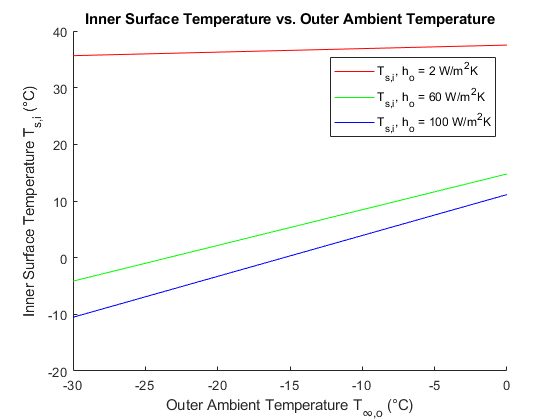
\includegraphics[width=0.8\textwidth]{io.png}
  \caption{Inner Surface Temperature vs. Outer Ambient Temperature}
\end{figure}

\begin{figure}[h!]
  \centering
  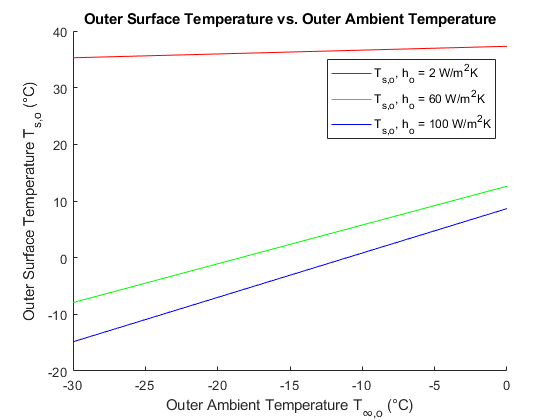
\includegraphics[width=0.8\textwidth]{oo.png}
  \caption{Outer Surface Temperature vs. Outer Ambient Temperature}
\end{figure}
\newpage

\newpage
\section*{Problem \#2}

\begin{center}
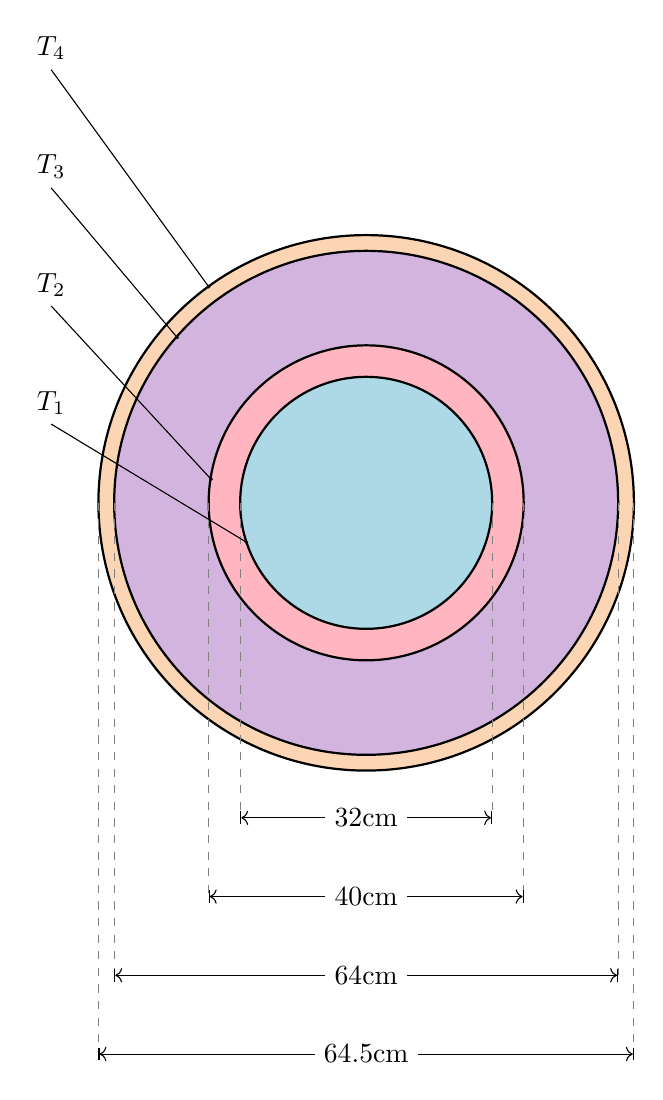
\begin{tikzpicture}[scale=0.1] % Scale down for the diagram to fit in the document.

    % Adding a grid for reference (adjust range and step as needed)
   % \draw[step=5.0, gray, very thin] (-100, -100) grid (100, 100); % Grid lines every 10 units

    % Outermost circle (exaggerated size for visibility)
    \draw[fill=orangecolor, thick] (0,0) circle (34cm); % 68cm diameter
    % Second circle
    \draw[fill=purplecolor, thick] (0,0) circle (32cm); % 64cm diameter
    % Third circle
    \draw[fill=pinkcolor, thick] (0,0) circle (20cm); % 40cm diameter
    % Innermost circle
    \draw[fill=bluecolor, thick] (0,0) circle (16cm); % 32cm diameter
    
    % Vertical guide lines for each circle
    \draw[dashed, gray] (34,0) -- (34,-70); % To edge of outermost circle
    \draw[dashed, gray] (-34,0) -- (-34,-70); % From outermost dimension line to edge
    \draw[dashed, gray] (-32,0) -- (-32,-60); % To edge of second circle
    \draw[dashed, gray] (32,0) -- (32,-60); % From third circle dimension line to edge
    \draw[dashed, gray] (20,0) -- (20,-50); % To edge of innermost circle
    \draw[dashed, gray] (-20,0) -- (-20,-50); % From innermost dimension line to edge
    \draw[dashed, gray] (16,0) -- (16,-40); % To edge of innermost circle
    \draw[dashed, gray] (-16,0) -- (-16,-40); % From innermost dimension line to edge
    
    % Dimensions
    % For outermost circle
    \draw[|<->|] (-34,-70) -- (34,-70) node[midway, fill=white] {64.5cm};
    % For second circle
    \draw[|<->|] (-32,-60) -- (32,-60) node[midway, fill=white] {64cm};
    % For third circle
    \draw[|<->|] (-20,-50) -- (20,-50) node[midway, fill=white] {40cm};
    % For innermost circle
    \draw[|<->|] (-16,-40) -- (16,-40) node[midway, fill=white] {32cm};

    % Line that starts with a small circle and ends with text
    \draw[] (-20,27.45) -- node[at start, circle, fill, inner sep=0.5pt] {} node[at end, above] {$T_4$} (-40, 55);
    \draw[] (-24,21) -- node[at start, circle, fill, inner sep=0.5pt] {} node[at end, above] {$T_3$} (-40, 40);
    \draw[] (-19.7,3) -- node[at start, circle, fill, inner sep=0.5pt] {} node[at end, above] {$T_2$} (-40, 25);
    \draw[] (-15.2,-5) -- node[at start, circle, fill, inner sep=0.5pt] {} node[at end, above] {$T_1$} (-40, 10);

\end{tikzpicture}

\begin{circuitikz}[american resistors, thick]
\tikzstyle{every node}=[font=\large]
% Defining the thermal resistances
\draw (0,-1) to[R, l=$R_1$, -*] (3,-1) 
      (3,-1) to[R, l=$R_2$, -*] (7,-1)
      (7,-1) to[R, l=$R_3$, -*] (10,-1)
      
      (10,-0.5) to[short] (10,-1.5)
      (10,-1.5) to[R, l=$R_5$, -] (13,-1.5)
      (10,-0.5) to[R, l=$R_4$, -] (13,-0.5)
      (13,-0.5) to[short] (13,-1.5)
      (13,-1) to[short, *-] (14,-1);

% Adding the input and output labels
\node at (-0.8,-1) {Tin};
\node at (15,-1) {Tout};
\end{circuitikz}
\end{center}

\subsection*{Steel Pipe}
The thermal resistance of the steel pipe (\(R_1\)) is determined by its material properties and geometric dimensions. The formula used is:

\[
R_1 = \frac{\ln(\frac{r_o}{r_i})}{2 \pi k_{steel} L}
\]

where:
\begin{itemize}
    \item \(r_o = 0.20\) m is the outer radius,
    \item \(r_i = 0.16\) m is the inner radius,
    \item \(k_{steel} = 40\) W/(m K) is the thermal conductivity,
    \item \(L = 1\) m is the length of the pipe (for per meter calculations).
\end{itemize}

Substituting the known values, the thermal resistance of the steel pipe is calculated as:

\[
R_1 = \frac{\ln(\frac{0.20}{0.16})}{2 \pi \times 40 \times 1} \approx 0.00089 \, \text{m}^2\text{K/W}
\]

\subsection*{Calcium Silicate Insulation}
The thermal resistance of the calcium silicate insulation (\(R_2\)) depends on its thermal conductivity and the dimensions of the insulation layer. The relevant formula is:

\[
R_2 = \frac{\ln(\frac{r_{o,ins}}{r_{i,ins}})}{2 \pi k_{ins} L}
\]

where:
\begin{itemize}
    \item \(r_{o,ins} = 0.32\) m is the outer radius of the insulation,
    \item \(r_{i,ins} = 0.20\) m is the inner radius of the insulation (equal to the outer radius of the steel pipe),
    \item \(k_{ins} = 0.092\) W/(m K) is the thermal conductivity of the calcium silicate,
    \item \(L = 1\) m is the length of the pipe section we are considering.
\end{itemize}

Inserting these values, the thermal resistance of the calcium silicate insulation layer is calculated as follows:

\[
R_2 = \frac{\ln(\frac{0.32}{0.20})}{2 \pi \times 0.092 \times 1} \approx 0.81308 \, \text{m}^2\text{K/W}
\]

\subsection*{Aluminum Sheet}
The thermal resistance of the aluminum sheet (\(R_3\)) also relies on its material properties and dimensions but is usually quite small due to aluminum's high thermal conductivity. The resistance is given by:

\[
R_3 = \frac{\ln(\frac{r_{o,alu}}{r_{i,alu}})}{2 \pi k_{alu} L}
\]

where:
\begin{itemize}
    \item \(r_{o,alu} = 0.3225\) m is the outer radius of the aluminum sheet,
    \item \(r_{i,alu} = 0.32\) m is the inner radius of the aluminum sheet (equal to the outer radius of the insulation),
    \item \(k_{alu} = 170\) W/(m K) is the thermal conductivity of aluminum,
    \item \(L = 1\) m represents the length for our per-meter calculation.
\end{itemize}

Inserting the values into the equation, the thermal resistance for the aluminum sheet is found to be:

\[
R_3 = \frac{\ln(\frac{0.3225}{0.32})}{2 \pi \times 170 \times 1} \approx 0.00000729 \, \text{m}^2\text{K/W}
\]

\subsection*{Convective Heat Transfer}
The thermal resistance due to convection from the aluminum sheet's surface to the ambient air (\(R_c\)) is critical for understanding the heat loss from the pipe's exterior. It is calculated as follows:

\[
R_c = \frac{1}{h_c A}
\]

where:
\begin{itemize}
    \item \(h_c = 11\) W/(m\(^2\)K) represents the convective heat transfer coefficient between the aluminum surface and the ambient air,
    \item \(A = 2 \pi r_{o,alu} L\) is the outer surface area of the aluminum per meter of pipe length, with \(r_{o,alu} = 0.3225\) m and \(L = 1\) m.
\end{itemize}

By substituting the known values into the equation, the convective thermal resistance is calculated:

\[
R_c = \frac{1}{11 \times 2 \pi \times 0.3225 \times 1} \approx 0.04486 \, \text{m}^2\text{K/W}
\]

\subsection*{Radiative Heat Transfer}
In addition to convection, radiative heat transfer from the aluminum surface to the surroundings also contributes to heat loss. The thermal resistance due to radiation (\(R_r\)) is given by:

\[
R_r = \frac{1}{\epsilon \sigma T_{average}^3 A}
\]

where:
\begin{itemize}
    \item \(\epsilon = 0.1\) is the emissivity of the aluminum surface,
    \item \(\sigma = 5.67 \times 10^{-8}\) W/(m\(^2\)K\(^4\)) is the Stefan-Boltzmann constant,
    \item \(T_{average}\) is the average temperature of the surface in Kelvin, assumed here as the ambient temperature (26°C or 299.15 K for simplification),
    \item \(A = 2 \pi r_{o,alu} L\) as before.
\end{itemize}

With these parameters, the radiative thermal resistance is:

\[
R_r = \frac{1}{0.1 \times 5.67 \times 10^{-8} \times (299.15)^3 \times 2 \pi \times 0.3225 \times 1} \approx 0.8128 \, \text{m}^2\text{K/W}
\]
\subsection*{Final Calculation of Total Thermal Resistance}
Inserting the calculated values into the total thermal resistance equation, we obtain:

\[
R_{total} = 0.00089 \, \text{m}^2\text{K/W} + 0.81308 \, \text{m}^2\text{K/W} + 0.00000729 \, \text{m}^2\text{K/W} + \left(\frac{1}{0.04486 \, \text{m}^2\text{K/W}} + \frac{1}{0.8128 \, \text{m}^2\text{K/W}}\right)^{-1} 
\]
\[
\approx 0.8565 \, \text{m}^2\text{K/W}
\]

This total thermal resistance encompasses the effects of conduction through each layer and the combined effects of convection and radiation from the exterior surface.

\subsection*{Final Calculation of Heat Loss Per Meter}
With the total thermal resistance determined, the heat loss per meter can be calculated as follows:

\[
Q/L = \frac{\Delta T}{R_{total}} = \frac{539}{0.8565} \approx 629.31 \, \text{W/m}
\]

This result represents the heat loss per meter length from the steam pipe, factoring in all mechanisms of heat transfer including conduction, convection, and radiation.

\newpage
\section*{Problem \#3}
The wall is constructed as follows:
\begin{itemize}
    \item Hardwood siding: 8 mm thick
    \item Hardwood studs: 40 mm by 130 mm, spaced on 0.65 m centers
    \item Glass fiber insulation (paper faced, 28 kg/m$^3$): fills the space between the studs
    \item Gypsum (vermiculite) wall board: 12 mm thick
\end{itemize}
Thermal conductivities at $\approx$300K:
\begin{align*}
    k_A &= 0.094 \text{ W/m$\cdot$K} \quad \text{(Hardwood siding)} \\
    k_B &= 0.16 \text{ W/m$\cdot$K} \quad \text{(Hardwood)} \\
    k_C &= 0.17 \text{ W/m$\cdot$K} \quad \text{(Gypsum)} \\
    k_D &= 0.038 \text{ W/m$\cdot$K} \quad \text{(Insulation)}
\end{align*}

\begin{center}
\begin{circuitikz}[american resistors, thick]
\tikzstyle{every node}=[font=\large]
% Defining the thermal resistances
\draw (0,-1) to[R, l=$A$, -*] (3,-1) 
      (3,0) to[short] (3,-2)
      (3,-2) to[R, l=$D$, -] (7,-2)
      (3,0) to[R, l=$B$, -] (7,0)
      (7,0) to[short] (7,-2)
      (7,-1) to[R, l=$C$, *-] (10,-1);

% Adding the input and output labels
\node at (-0.8,-1) {Input};
\node at (11,-1) {Output};
\end{circuitikz}
\end{center}

The thermal resistance for the hardwood siding ($R_A$) is calculated as:
\[ R_A = \frac{L_A}{k_A A_{total}} \]
where $L_A = 8 \times 10^{-3}$ m is the thickness, $k_A = 0.094$ W/m$\cdot$K is the thermal conductivity, and $A_{total}$ is the total area of the wall.
\newline\newline
The thermal resistance for the hardwood studs ($R_B$), considering all studs together, is calculated as:
\[ R_B = \frac{L_B}{k_B A_{stud}} \]
where $L_B = 130 \times 10^{-3}$ m is the thickness, $k_B = 0.16$ W/m$\cdot$K is the thermal conductivity, and $A_{stud}$ is the area of all studs.
\newline\newline
The thermal resistance for the glass fiber insulation ($R_D$) is calculated as:
\[ R_D = \frac{L_D}{k_D (A_{total} - A_{total\_studs})} \]
where $L_D = 130 \times 10^{-3}$ m is the thickness, $k_D = 0.038$ W/m$\cdot$K is the thermal conductivity, and $A_{total\_studs}$ is the total area taken up by the studs.
\newline\newline
The thermal resistance for the gypsum wall board ($R_C$) is calculated as:
\[ R_C = \frac{L_C}{k_C A_{total}} \]
where $L_C = 12 \times 10^{-3}$ m is the thickness, and $k_C = 0.17$ W/m$\cdot$K is the thermal conductivity.
\newline\newline
The total thermal resistance ($R_{total}$) for the wall is calculated by combining the resistances in series and parallel:
\[ R_{total} = R_A + R_C + ( \frac{1}{\frac{1}{R_B} + \frac{1}{R_D}}) \]
\[ R_{total} \approx 1.8538 K/W\]

\newpage
\section*{Problem \#4}
This document details the calculations for the heat dissipation from a cylindrical aluminum pin fin, given the following parameters:
\begin{itemize}
    \item Diameter of the fin: 4 mm
    \item Length of the fin: 20 mm
    \item Base temperature: 600 K
    \item Fluid temperature: 400 K
    \item Heat transfer coefficient: $100 \, \text{W/(m}^2\text{K)}$
    \item Thermal conductivity of aluminum: $180 \, \text{W/(m K)}$
\end{itemize}

\begin{center}
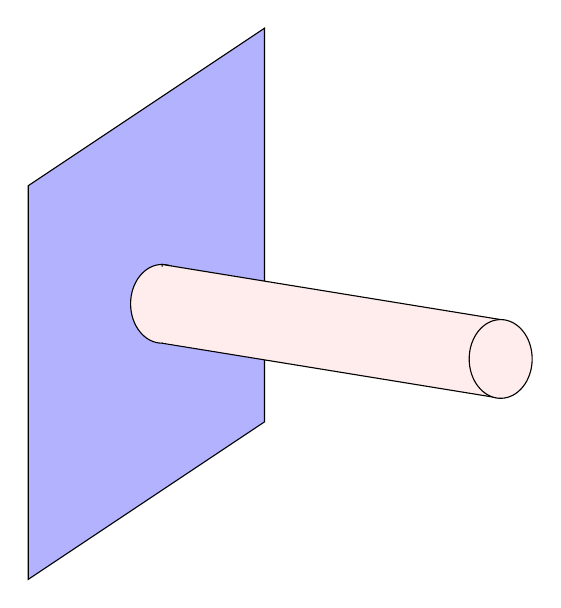
\begin{tikzpicture}
    % Draw the filled polygon
    \filldraw[fill=blue!30] (0,-2) -- (3,0) -- (3,-5) -- (0,-7) -- cycle;
    
    % Draw the first ellipse
    \filldraw[fill=pink!30] (1.7,-3.5) ellipse (0.4 and 0.5); % Width is 0.8 of height, so if height = 1, width = 0.8
    \filldraw[fill=pink!30] (1.7,-3.5+0.5) -- (6,-4.2+0.5) -- (6,-4.2-0.5) -- (1.7,-3.5-0.5) -- cycle;
    % Draw the second ellipse
    \filldraw[fill=pink!30] (6,-4.2) ellipse (0.4 and 0.5); % Same dimensions as the first ellipse

    % Draw the connecting rectangle (represents the body of the cylinder)
    \fill[pink!30] (1.65,-3.5+0.48) -- (5,-4.2+0.48) -- (5,-4.2-0.31) -- (1.65,-3.5-0.48) -- cycle;

\end{tikzpicture}
\end{center}

\subsection*{Calculation of Perimeter and Area}
The perimeter (P) and cross-sectional area (A) of the cylindrical fin are calculated as follows:
\begin{align}
    P &= 2\pi R = 2\pi \times 2 \times 10^{-3} \, \text{m} \\
    A &= \pi R^2 = \pi \times (2 \times 10^{-3})^2 \, \text{m}^2
\end{align}
The calculated values are:
\begin{itemize}
    \item Perimeter, $P = 0.01257 \, \text{m}$
    \item Area, $A = 1.2566 \times 10^{-5} \, \text{m}^2$
\end{itemize}

\subsection*{Calculation of Beta ($\beta$)}
The parameter $\beta$, which reflects the geometry and thermal properties of the fin, is given by:
\begin{equation}
    \beta = \sqrt{\frac{h \times P}{k \times A}}
\end{equation}
The calculated value of $\beta$ is approximately $23.57 \, \text{m}^{-1}$.

\subsection*{Calculation of $\beta$L}
The dimensionless parameter $\beta$ L is calculated as:
\begin{equation}
    \beta L = 23.57 \times 20 \times 10^{-3} = 0.471
\end{equation}
Since $\beta L < 3$, the fin is considered to have the characteristics of an "infinite" fin in terms of its heat transfer behavior.

\subsection*{Calculation of Heat Dissipation (\(Q_{fin}\))}
The heat dissipation from the fin, $Q_{fin}$, is calculated as follows:
\begin{equation}
    Q_{fin} = \sqrt{k \times h \times P \times A} \times (T_{base} - T_{\infty}) \times \tanh(\beta L)
\end{equation}
The calculated heat dissipation from the fin is approximately $4.685 \, \text{W}$.


\newpage
\section*{Problem \#5}
\subsection*{Coordinate System with Origin at the Fin Base}
The temperature distribution is governed by the differential equation:
\[
\frac{d^2T}{dx^2} - m^2(T - T_\infty) = 0,
\]
with boundary conditions: at $x = 0$, $T = T_b$, and at $x = L$, $\frac{dT}{dx} = 0$ (insulated tip).

The general solution is:
\[
T(x) = C_1 \cosh(mx) + C_2 \sinh(mx) + T_\infty.
\]
Applying the boundary conditions:
At $x = 0$: $T_b = C_1 + T_\infty$, so $C_1 = T_b - T_\infty$.
At $x = L$: $0 = mC_1 \sinh(mL) + mC_2 \cosh(mL)$, leading to $C_2 = -C_1 \tanh(mL)$.
The temperature distribution then becomes:
\[
T(x) = (T_b - T_\infty) \left[\cosh(mx) - \tanh(mL) \sinh(mx)\right] + T_\infty.
\]
The total heat transfer rate from the fin, $Q$, is:
\[
Q = kA_c m (T_b - T_\infty) \tanh(mL).
\]

\subsection*{Coordinate System with Origin at the Fin Tip}
In this system, we denote the position by $x' = L - x$. The heat conduction equation remains the same but applies to the new coordinate $x'$:
\[
\frac{d^2T}{dx'^2} - m^2(T - T_\infty) = 0.
\]
The boundary conditions are: at $x' = L$, $T = T_b$, and at $x' = 0$, $\frac{dT}{dx'} = 0$ (insulated tip).

Following similar steps, the solution to the differential equation is:
\[
T(x') = C_1' \cosh(mx') + C_2' \sinh(mx') + T_\infty,
\]
with $C_2' = 0$ from the boundary condition at $x' = 0$ and $C_1' = (T_b - T_\infty) / \cosh(mL)$ from the condition at $x' = L$.
Therefore, the temperature distribution is:
\[
T(x') = \frac{(T_b - T_\infty)}{\cosh(mL)} \cosh(mx') + T_\infty.
\]
The total heat transfer rate, $Q$, remains unchanged from the base-oriented system as:
\[
Q = kA_c m (T_b - T_\infty) \tanh(mL).
\]

\end{document}
